\chapter{Un profil UML pour aider à la rédaction de GDD: \emph{Game Genesis}}
\label{game-genesis.sect}

%GDD
Le \emph{Game Design Document}, comme décrit dans la Section~\ref{sect.GDD}, permet de réunir toutes les informations de design nécessaires au développement d'un jeu vidéo. La structure du GDD est définie en respectant des bonnes pratiques et selon les besoins de design du jeu concerné.


\gt{Ci-bas: il faut \^etre plus sp\'ecifique pour l'aspect Mechanics
car si tu dis <<{\bf tous} les \'el\'ements du jeu>>, alors pourquoi
faudrait-il autre chose que cela!?}

%MDA
Le \emph{Framework Mechanics, Dynamics, Aesthetics}, comme décrit dans le Chapitre~\ref{chap.MDA}, permet de séparer les différents aspects du design d'un jeu vidéo. L'aspect \emph{Mechanics} permet de représenter les éléments du jeu rattachés aux données et aux algorithmes, l'aspect \emph{Dynamics} décrit le comportement des \'el\'ements de \emph{Mechanics}, alors que l'aspect \emph{Aesthetics} d\'ecrit les émotions découlant de la \emph{Dynamics} que le jeu génère chez le joueur.

%UML
Les profils UML, décrits dans le Chapitre~\ref{chap.profils-UML}, permettent d'étendre les concepts présents dans UML. Mettre en place un profil UML permet de faciliter la cr\'eation d'un modèle et de son contenu pour un domaine particulier. Un profil se compose de stéréotypes, de valeurs étiquetées et de contraintes, qui ensemble permettent de d\'efinir de nouveaux concepts utilisables dans la description de modèles.


\section{Un aper\c{c}u de \emph{Game Genesis}}
\label{sect.gg_what}
%quoi
\emph{Game Genesis} est un profil UML que nous avons d\'evelopp\'e et qui permet d'adapter UML au domaine du design de jeu vidéos. 
Plus précisément, \emph{Game Genesis} introduits de nouvelles classes UML --- par le biais de st\'er\'eotypes --- afin de l'adapter à la rédaction d'un GDD.


\gt{Ci-bas et ailleurs. Je ne crois pas que tu devrais utiliser
directement le terme Mechanics comme dans <<un certain nombre de
Mechanics>>.  Comme indiqu\'e pr\'ec\'edemment (vieille remarque GT),
il me semble que Mechanics, en anglais, est plus compris au sens de
<<la m\'ecanique>> --- m\'ecanique des fluides, m\'ecanique quantique,
etc.  C'est pour cela que, plus haut, j'ai chang\'e pour <<l'aspect
Mechanics>>, que ci-bas j'ai indiqu\'e <<\'el\'ements de Mechanics>>.}

\gt{Et je viens de regarder l'article initial sur MDA.  L\`a aussi,
les termes Mechanics, Dynamics et Aesthetics sont consid\'er\'es comme
des substantifs au singulier: <<Mechanics describes the particular
components of the game, ...>>, <<Dynamics describes the run-time
behavior...>>, <<Aesthetics describes...>>.}


\gt{Et le terme <<aspect>> me semble aussi appropri\'e --- bien que
celui de <<vue>> ou <<point de vue>> pourrait aussi l'\^etre: <<Each
component of the MDA framework can be thought of as a 'lens' or a
'view' of the game...>>.}



Afin de rédiger un GDD, un \emph{game designer} doit d'abord définir les bases du jeu.
Durant cette étape le \emph{game designer} va devoir définir un certain nombre d'\'el\'ements de \emph{Mechanics} qui correspondent aux objets présents dans le jeu ainsi que leurs actions et interactions.
Ces \'el\'ements de \emph{Mechanics} peuvent aussi bien être des objets visibles dans le jeu --- comme des personnages, des ennemis, des armes, des bâtiments --- mais également des \'el\'ements autour du jeu --- comme des cartes, des chronomètres, des statistiques, etc.
Tous ces \'el\'ements de \emph{Mechanics} ont des caractéristiques communes et des caractéristiques qui leur sont propres.

%comment
\emph{Game Genesis} permet à un \emph{game designer} de répertorier et décrire ces \'el\'ements de \emph{Mechanics} sous forme de diagrammes de classes.
Chaque catégorie de \emph{Mechanics} est représenté par une classe, et
chaque \'el\'ement de \emph{Mechanics} est aussi représenté par une classe.
L'appartenance à une catégorie est définie par des relations d'héritage.
Les caractéristiques des catégories et des divers \'el\'ements de \emph{Mechanics} sont représentées par des attributs des classes.
Finalement, les interactions possibles entre \'el\'ements du jeu sont représentées par des associations entre classes, associations auxquelles sont parfois associ\'ees diverses contraintes.

%pourquoi
L'utilisation de diagrammes de classes UML apporte certain avantages pour la modélisation des \'el\'ements de \emph{Mechanics}:
\begin{itemize}
    \item Structure
    \item Langage de modélisation formel et normalisé
    \item Support de communication visuel \gt{Pas trop certain de ce que cela veut dire, i.e., un peu vague: <<performant>>!}
    \item Utilisation d'outils adaptés
    \item Facilement versionnable
    \item Assez souple pour s'adapter aux domaines ou aux plateformes de développement \gt{s'adapter \`a quoi!?}
\end{itemize}

Cependant, UML est un langage avant tout destiné à modéliser les systèmes informatiques et les processus d'affaire. 
Il est donc nécessaire de l'adapter afin de lui apporter le vocabulaire et les logiques nécessaires à la description de l'aspect \emph{Mechanics} d'un jeu vidéo.
C'est à cela que sert le profil \emph{Game Genesis}.
   




\section{\emph{Game Genesis} en détail}

\emph{Game Genesis} est un profil UML permettant d'adapter un diagramme de classe pour la rédaction d'un GDD.
Dans les sections ci-dessous nous allons définir les éléments suivants :
\begin{itemize}
    \item Les stéréotypes afin d'étendre les classes,
    \item Les stéréotypes afin d'étendre les associations,
    \item Les contraintes afin de définir des règles d'utilisation des stéréotypes.
\end{itemize}

\subsection{Stéréotypes}

\gt{Dans la figure, comme ce sont des \'el\'ements de <<code>> ---
classes UML --- il vaut mieux utiliser la police teletype.}

\gt{Ce serait pr\'ef\'erable que dans les deux parties de la figure,
les r\'ef\'erences aux annexes soient pr\'esent\'ees de la m\^eme
fa\c{c}on pouar Animate, Lore, World et Interaction. Sinon, cela donne
l'impression que la s\'emantique pourrait \^etre diff\'erente ---
parce que c'est bien la m\^eme, n'est-ce pas?}

\begin{figure}
    \begin{adjustbox}{width=\linewidth}
        \begin{forest}
         [\texttt{Game Genesis}
         [\texttt{Item}
             [\texttt{Wearable},tier=2
                 [\texttt{Weapon},tier=before
                    [Fig.~\ref{A-Weapon},tier=bottom]
                 ]
                 [\texttt{Equipment},tier=before
                    [Fig.~\ref{A-Equipment},tier=bottom]
                 ]
                 [\texttt{Jewerly},tier=before
                    [Fig.~\ref{A-Jewerly},tier=bottom]
                 ]
                 [\texttt{Tool},tier=before
                    [Fig.~\ref{A-Tool},tier=bottom]
                 ]
             ]
             [\texttt{Add-on},tier=2
                    [Fig.~\ref{A-Add-on},tier=bottom]
             ]
             [\texttt{Usable},tier=2
                    [Fig.~\ref{A-Usable},tier=bottom]
             ]
             [\texttt{Craft},tier=2
                    [Fig.~\ref{A-Craft},tier=bottom]
            ]
             [\texttt{Currency},tier=2
                    [Fig.~\ref{A-Currency},tier=bottom]
            ]
         ]
         ]
        \end{forest}
    \end{adjustbox}
    \caption{Arbre des stéréotypes de \emph{Game Genesis}.}
    \label{fig.GG}
\end{figure}
    
\begin{figure}
    \begin{adjustbox}{width=\linewidth}
        \begin{forest}
         [\texttt{Game Genesis}
         [\texttt{Animate} ,tier=2
                [Fig.\ref{A-Animate},tier=bottom]
         ]
         [\texttt{CharacterSheet},tier=2
                [\texttt{Statistic},tier=before
                    [Fig.~\ref{A-Statistic},tier=bottom]
                ]
                [\texttt{Attribute},tier=before
                    [Fig.~\ref{A-Attribute},tier=bottom]
                ]
                [\texttt{Information},tier=before
                    [Fig.~\ref{A-Information},tier=bottom]
                ]
                [\texttt{Experience},tier=before]
                [\texttt{Ability},tier=before]
         ]
         [\texttt{Lore} ,tier=2
                [Fig.~\ref{A-Lore},tier=bottom]
         ]
         [\texttt{World} ,tier=2
                [Fig.~\ref{A-World},tier=bottom]
         ]
         [\texttt{Interaction},tier=2
                [Fig.~\ref{A-Interaction},tier=bottom]
         ]
         ]
        \end{forest}
    \end{adjustbox}
    \caption{Arbre des stéréotypes de \emph{Game Genesis} (suite).}
    \label{fig.GG2}
\end{figure}


\gt{Ci-bas: dans le cas pr\'esent, ce n'est pas tant une
<<red\'efinition>> qu'une extension, qu'une cr\'eation de nouvelles
classes, de nouveaux concepts! Donc, j'ai modifi\'e en cons\'equence.}

Dans la Section~\ref{sect.uml.ster}, nous avons décrit le mécanisme de d'extension de metaclass afin d'introduire de nouveaux concepts par le biais des Stéréotypes. 
Dans \emph{Game Genesis}, nous faisons donc usage des stéréotypes afin d'étendre les classes d'un modèle de jeu et ainsi permettre la rédaction de GDD.
Dans un article de Salazar \emph{et al.}~\cite{GDD_software}, plus particulièrement dans la documentation additionnelle de cet article~\cite{salazar_gdd}, nous avons identifié un certain nombre d'\'el\'ements de \emph{Mechanics} typiquement présents dans un GDD.
Nous avons constaté que tous les éléments étaient répartis dans des catégories possédant elles-mêmes certaines caractéristiques communes. 
Nous avons extrait les catégories suivantes :

\begin{itemize}
    \item Player Character
    \item Non Player Character
    \item Enemy
    \item Final Enemy
    \item Help Object
    \item Extra Object
    \item Other Object
\end{itemize}


\gt{Ci-haut: Si ce sont des noms de classes, pr\'esents dans le
mod\`ele/profil UML, alors il faut utiliser la convention des noms de
classe UML, i.e., un seul <<mot>> en CamelCase: PlayerCharacter,
FinalEnemy, etc.}
\EH{J'ai enlevé le txt teletype dans cet itemize car ce sont des éléments présents dans l'exemple de GDD Donkey Kong de l'article (sous forme textuel) et non pas des éléments du profil qui sont cités}

Les classes UML fonctionnent avec un système d'héritage de classes.
La classe enfant hérite des attributs et méthodes de la classe parent.
Dans un GDD, un \'el\'ement de \emph{Mechanics} hérite des attributs énoncés dans les catégories parentes.
C'est ainsi que nous avons décidé d'utiliser un diagramme de classes afin de représenter les \emph{Mechanics} comme des classes et de spécifier leurs caractéristiques dans les attributs.
%
\gt{Je crois que les phrases qui suivent sont redondantes, n'apportent
rien de plus. Sinon, il faut les reformuler, car je ne comprends pas
bien ce qu'elles introduisent de nouveau.}
\eh{Supprimées}
%
\begin{figure}
    \centering
    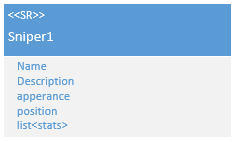
\includegraphics[width=5cm]{10_img/chap5/sniper.PNG} 
    \caption{Héritage d'une classe \texttt{Sniper1} utilisant le stéréotype \texttt{SR}.}
    \label{fig.sniper}
\end{figure}

\gt{Idem pour ce qui suit!}
%

La figure~\ref{fig.sniper} pr\'esente un exemple d'une classe \texttt{Sniper1}, un élément de \emph{Mechanics} du GDD d\'efini avec le profil \emph{Game Genesis}.
Nous voyons que la classe hérite ainsi des attributs des Stéréotypes précédents dans la logique d'héritage de classes.
Dans son implémentation la classe <<~Sniper1~>> possèdera les attributes des stéréotypes <<~Item~>>, <<~Wearable~>>, <<~Weapon~>> et <<~SR~>>.

\gt{Ci-haut et dans la figure: non, ce n'est pas ainsi qu'il faut
pr\'esenter cela il me semble. Plusieurs remarques. 1) Ce serait bien
de toujours distinguer, par les couleurs, la sp\'ecification du profil
(bleu!) de son utilisation (vert!). Or, la sp\'ecification de Sniper1
est une utilisation.  2) Si tu mets directement les d\'etails dans la
boite Sniper1, alors c'est comme si l'usager les sp\'ecifiait
lui-m\^eme. Or, ici, de ce que je comprends, tu essaies d'expliquer
qu'il y a h\'eritage implicite.  Une possibilit\'e serait de mettre en
vert une boite avec <<SR>> et Sniper, sans attributs, puis juste \`a
cot\'e de mettre une boite (autre couleur?) avec juste Sniper comme
nom mais o\`u tous les attributs sont maintenant pr\'esents ---
justement \`a cause de l'h\'eritage {\bf implicite} associ\'e \`a ta
hi\'erarchie de st\'er\'eotypes.}

\gt{En d'autres mots, il me semble que tu dois insister plus sur le
fait que la sp\'ecification d'un st\'er\'eotype introduit un nouveau
{\bf concept} --- une nouvelle classe ---, lequel concept peut
\'evidemment poss\'eder des attributs --- indiqu\'es directement (dans
sa boite) ou indirectement (via h\'eritage).  Une fois ce concept
d\'efini, on peut ensuite l'utiliser pour d\'efinir de nouvelles
classes, dont les objets poss\`edent tous les attributs associ\'es au
concept --- peu importe d'o\`u proviennent ces attributs (directs ou
indirects).}

\GT{De plus, puisque tu as un exemple d'utilisation du st\'er\'eotype
SR, tu devrais aussi donner un exemple de sp\'ecification/utilisation
des valeurs \'etiquet\'ees pour sp\'ecifier des attributs.}



\subsection{Interactions}
Les éléments de \emph{Mechanics} ne sont pas tous des éléments isolés et une expérience de jeu ne serait rien sans les interactions que le joueur peut avoir avec les divers \'el\'ements du jeu.
Ces interactions sont présentées dans le gabarit de GDD de Salazar \emph{et al.}~\cite{salazar_gdd} sous forme de règles d'interaction.
Ces règles sont composées de divers éléments, notamment les suivants :
\begin{itemize}
    \item Deux \'el\'ements (ou plus) de \emph{Mechanics} 
    \item Une interaction entre ces \'el\'ements
    \item Une contrainte appliquée à cette interaction (optionnelle)
\end{itemize}
Les interactions que nous avons identifi\'ees comme int\'eressantes sont les suivantes --- voir aussi la Figure~\ref{A-Interaction}~:
\begin{itemize}
\item \texttt{Attack}
\item \ACOMPLETER{Donner ici la liste des noms des diverses interactions que tu as identifi\'ees}
\item 
\end{itemize}


\GT{Il faut aussi que tu montres clairement, parce que c'est dans le
contexte d'un profil UML, qu'il s'agit d'extension de la Metaclass
fAssociation d'UML --- comme \'evoqu\'e l'autre fois (quand on s'est
rencontr\'es? je ne suis plus certain.}

\GT{Idem pour les st\'er\'eotypes de classes de la section
pr\'ec\'edente: on devrait voir ici -- et possiblement aussi dans
l'annexe --- qu'il s'agit d'extension de la Metaclass Class!}

\subsection{Contraintes}

\GT{Quelques contraintes? Ou pas? Ce serait bien d'en d\'ecrire un
certain nombre, ne serait-ce que pour illustrer le principe que les
interactions ne sont pas entre n'importe quels items.}


\section{Conclusion}


%%%%%%%%%%%%%%%%%%%%%%%%%%%%%%%%%%%%%%%%%%%%%%%%%%%%%%%%%%%%%%%%%%%%%%%%%%
\begin{comment}
\chapter{Un langage de modélisation pour l'établissement d'un Game Design Document}

\section{Le concept}
\subsection{Définition}
\subsubsection{Quoi ?}
Un langage permettant de modéliser et stocker des idées lors des phases de Breakthrough et de Conception d'un projet de jeu vidéo. La modélisation peut être graphique et/ou textuelle avec application des modifications en parallèle. \\
Les informations peuvent contenir tout le nécessaire pour exprimer les idées (textes, informations numériques, chemins de fichiers...). Les champs peuvent être personalisables pour permettre de la souplesse aux utilisateurs.

\subsubsection{Pour quoi faire ?}
\paragraph{Des outils de modélisation existent pour tous les domaines reliés au développement de logiciels. Ils sont souvent spécifiques à un corps de métier afin de pouvoir proposer un maximum de fonctionnalités spécifiques sans devenir trop compliqué et en utilisant un vocabulaire précis qui correspond au corps de métier concerné.}

\paragraph{Il y a peu ou pas de langages de modélisation plus généraux pour des domaines multi-métiers. Le but est de pouvoir modéliser la réflexion créative en fournissant un élément visuel permettant de mind-mapper les idées, les stocker et les réutiliser. \\
Il faut que la modélisation soit assez souple pour pouvoir répondre aux besoins de chacun des corps de métier d'où le fait que les éléments et attributs peuvent avoir des identifiants spécifiques définis librement par l'utilisateur.}

\subsubsection{Pour quelles raisons ?}
\paragraph{Les supports de réflexion actuellement utilisés : cahier des charges, réunions, notes écrites, mails, minds-maps... L'organisation de ces différents supports dans un ensemble cohérent est tr;s compliqué. Dans un cahier des charges il est compliqué de classer les idées à la volée. Un mind-map nécessite une numérisation ou une retranscription sur un outil de mind-mapping qui sont toutes les deux des techniques non péreines et risquées dans la conservation des données. Des notes écrites peuvent se perdre et n'ont pas de durabilité sur le long terme. Des mails sont péreins mais il est difficile de les organiser pour le stockage de l'information.}
\paragraph{Un langage de modélisation graphique et textuel permettrait de mind-mapper les idées à la volée sous forme de cubes contenant les données nécessaires. La hiérarchisation des éléments permettrait de gérer des héritages et des relations ainsi que d'éviter la répétition trop abondante des mêmes informations. Les faces des cubes permettrait d'isoler les informations nécessaires à chacun des corps de métier.}
\end{comment}
